\documentclass[runningheads]{llncs}
\usepackage{graphicx} % Required for inserting images
\usepackage{amsmath}   % for math environments
\usepackage{amssymb}
\usepackage{algorithm}
\usepackage{algpseudocode}
\usepackage{tabularx}
\usepackage{booktabs} % put this in the preamble
\usepackage{cancel}
\usepackage{float}
\usepackage{xcolor}
\usepackage{url}
\usepackage[utf8]{inputenc}
\usepackage[T1]{fontenc}
\usepackage[section]{placeins}
\title{Reducing Transform overhead in NTT-Based Product Chains: Algorithms and Efficient Implementation}
\titlerunning{Reducing Transform overhead in NTT-Based Product Chains: Algorithms and Efficient Implementation}

\begin{document}

\maketitle

\begin{abstract}
The Number Theoretic Transform allows for efficient multiplication algorithms, due to converting multiplication in polynomial rings into hadamard products of vectors. We describe an optimization for computing the product of k polynomials in a fixed quotient ring $Z_{q}[x]/(x^n+1)$ where $q$ is NTT-friendly. Standard approaches require $3(k-1)$ Number Theoretic Transforms, but by performing all intermediate multiplications as Hadamard products in the spectral domain and deferring the inverse transform, we reduce this to $k+1$ transforms. We prove the correctness of this method via a generalized convolution theorem, analyze complexity, and present a CRT-based extension that applies the optimization to general polynomial multiplication where intermediate products grow in degree. We perform extensive experimental analysis of both of these methods over the goldilocks prime $2^{64}-2^{32}+1$, ensuring predicted transform counts and speedup factors are accurate. We then state on application of the  method to RSA Auditing, showing how integers can be represented as polynomials through blocking and predicting the speedup factor through transform count analysis.

\keywords{Number Theoretic Transform \and Polynomial Multiplication \and Chinese Remainder Theorem \and Repeated Multiplication \and RSA Auditing \and Lattice-Based Cryptograpy}
\end{abstract}


\section{Introduction}

The Fast Fourier Transform (FFT), introduced by Cooley and Tukey~\cite{cooley1965algorithm} in 1965, reduces the cost of evaluating a degree-$n$ polynomial at $n$ points from $O(n^2)$ to $O(n \log n)$ operations. Gentleman and Sande~\cite{gentleman1966fft} presented an equivalent decimation-in-frequency formulation shortly after, most commonly used in evaluation of the inverse transform. Pollard~\cite{pollard1971fft} introduced the Number Theoretic Transform (NTT) as a finite-field analogue by replacing complex roots of unity with primitive roots of unity modulo a prime $q$. The transform achieves the same asymptotic cost with exact integer arithmetic over $\mathbb{Z}_q$, eliminating the floating-point rounding errors of the complex FFT. Schönhage and Strassen~\cite{schonhage1971} applied NTT-based convolution to large-integer multiplication, yielding an $O(n \log n \log \log n)$ algorithm that remains the foundation of modern multi-precision arithmetic libraries.

The NTT has since become a core primitive across cryptography. In lattice-based cryptography, key operations reduce to polynomial multiplication in quotient rings of the form $\mathbb{Z}_q[x]/(x^n+1)$. The NTT makes these multiplications practical, with schemes such as CRYSTALS-Kyber~\cite{bos2018kyber} and CRYSTALS-Dilithium~\cite{ducas2018dilithium}, recently standardised by NIST, achieving competitive performance for key encapsulation and digital signatures respectively. The NTT has also found application in spectral modular arithmetic over large RSA moduli~\cite{saldamli2007spectral} and, as this paper demonstrates, in accelerating polynomial product chains that arise in diverse computational contexts.

A single polynomial multiplication via the NTT requires two forward transforms, one pointwise (Hadamard) product, and one inverse transform. When a
chain of k polynomials must be multiplied, the standard approach applies this three-transform pattern to each of the $k - 1$ individual multiplications, resulting in
$3(k -1)$ transforms in total.

We observe that this standard approach is wasteful when all polynomials reside in the same fixed-size quotient ring. Each intermediate result is transformed back to the coefficient domain via an inverse NTT, only to be immediately transformed forward again for the next multiplication. These intermediate inverse-forward pairs are redundant: since the Hadamard product of two spectral vectors is itself a valid spectral vector in the same ring, all intermediate multiplications can be performed entirely in the NTT domain, and the inverse transform can be deferred to the very end of the computation.

The closest prior work is Saldamlı and Koç's Spectral Modular Exponentiation~\cite{saldamli2007spectral}, which performs modular exponentiation entirely in the spectral domain. They note the same elimination of redundant transforms in a multiplicative chain. We take their method one step further by recognizing that the multiplicative chains elements can be distinct, and thus extending the method past exponentiation.

Our contributions 
\begin{itemize}
    \item We state the Generalized Convolution Theorem, proving its correctness and its use of $k+1$ transforms compared with the standard count of $3(k-1)$ transforms.
    \item We state the Fixed-Ring Delayed Inverse Algorithm, making use of the Generalized Convolution Theorem, and stating its speedup factor of $\frac{3(k-1)}{k+1}$. We consider the limitations of this method to only be applicable under a coefficient modulus.
    \item We make use of the Chinese Remainder Theorem to apply the Fixed-Ring Delayed Inverse Algorithm to the general $\mathbb{Z}/(x^n+1)$ ring, dubbing this the General Delayed Inverse Algorithm. We do this by performing NTTs over a modulus so large that modular reduction is not needed. 
    \item We state and prove the minimum modulus size such that the General Delayed Inverse Algorithm may work without error.
    \item We provide experimental validation over the Goldilocks prime $q = 2^{64} - 2^{32} + 1$, confirming the theoretical transform counts exactly and demonstrating measured speedups approaching 3× for large chain lengths.
    \item We consider one of the applications of this method, that being RSA auditing. The problem involves multiplying multiple ($\approx 64)$ large integers. By representing integers as polynomials through blocking, the General Delayed Inverse Algorithm becomes applicable.
\end{itemize}


\paragraph{Organization.} Section 2 reviews the Number Theoretic Transform, the convolution theorem, and the Chinese Remainder Theorem. Section 3 presents the standard pairwise and balanced product tree algorithms for chain multiplication. Section 4 presents the Delayed Inverse Algorithm, the Generalized Convolution Theorem, the Hybrid Delayed Inverse Product Tree, and the General Delayed Inverse Algorithm. Section 5 provides experimental evaluation. Section 6 discusses an application to mass RSA key auditing. Section 7 concludes.

\section{Background}

Here, we define and show the Number Theoretic Transform over $\mathbb{Z}/(x^n+1)$. We define which modulus are NTT-possible and NTT-friendly and we show how to perform Cooley-Tukey Style fast NTTs. On top of this, we state the convolution theorem, showing how NTTs are able to optimize products, and state the Chinese Remainder Theorem.

\begin{definition}

    The Number Theoretic Transform~\cite{pollard1971fft} is a variant of the discrete Fourier transform, where the root of unity is not complex but instead an integer over a modular ring. It can be seen as an exact discrete Fourier transform due to not requiring floating-point precision. Consider a polynomial with coefficients over the ring $\mathbb{Z} / q\mathbb{Z}$. We express this polynomial $a_0+a_1x+a_2x^{2}... +a_{n-1}x^{n-1}$ in the vector form.
$$A=\begin{pmatrix}
a_0 \\
a_1 \\
\vdots \\
a_{n-1}
    \end{pmatrix} $$
And its NTT as
$$NTT(A)=\hat{A}=\begin{pmatrix}
\hat{a}_0 \\
\hat{a}_1 \\
\vdots \\
\hat{a}_{n-1}
    \end{pmatrix}$$

The NTT of this vector where each element is in $\mathbb{Z} / q\mathbb{Z}$ is found by
$$\hat{a}_j=\sum_{i=0}^{n-1}a_{i}\,\psi^{i}\omega^{ij} \pmod{q}$$

Where $\psi$ is a primitive $2n$-th root of unity in $\mathbb{Z}_q$ satisfying $\psi^{2n} \equiv 1 \pmod{q}$ and $\psi^n \equiv -1 \pmod{q}$, and $\omega = \psi^2$ is the corresponding $n$-th root of unity, so that $\psi^i\omega^{ij} = \psi^{i(2j+1)}$.
\end{definition}

\begin{definition}
    We say that a certain choice of modulus is NTT-friendly if
    $$\psi^{2n}\equiv1 \pmod{q}$$
    $$\psi^{n}\equiv-1 \pmod{q}$$
    $$\psi^{k}\not\equiv1, \quad k<2n \pmod{q}$$

    This ensures $\psi$ is a primitive $2n$-th root of unity, which allows for FFT-simplifications. For this to be possible the modulus must be such that, if the modulus is decomposed to its prime factors
$$q=p_0^{m_0}\cdotp p_1^{m_1}\cdotp p_2^{m_2}...\cdotp p_{k}^{m_{k}} $$
    then, for the nth root of unity to exist, 2n must divide $GCD(p_{0}-1,p_1-1,...p_k-1)$
\end{definition}

Defining the NTT and NTT-friendly moduli as such allow us to create simplifications akin to the Cooley-Tukey FFT~\cite{cooley1965algorithm}.

$$\hat{a}_j=\sum_{i=0}^{n-1}a_{i}\psi^{i}\omega^{ij}=$$
$$\sum_{i=0}^{\frac{n}{2}-1}a_{2i}\psi^{2i}\omega^{2ij}+\sum_{i=0}^{\frac{n}{2}-1}a_{2i+1}\psi^{2i+1}\omega^{(2i+1)j}=$$
$$\sum_{i=0}^{\frac{n}{2}-1}a_{2i}\omega^{i}\omega^{2ij}+\psi\omega^{j}\sum_{i=0}^{\frac{n}{2}-1}a_{2i+1}\omega^{i}\omega^{2ij}$$

As $\psi^{n}\equiv-1$ for NTT-friendly moduli:

$$\hat{a}_j=\sum_{i=0}^{\frac{n}{2}-1}a_{2i}\omega^{i(2j+1)}+\psi\omega^{j}\sum_{i=0}^{\frac{n}{2}-1}a_{2i+1}\omega^{i(2j+1)}$$
$$\hat{a}_{j+\frac{n}{2}}=\sum_{i=0}^{\frac{n}{2}-1}a_{2i}\omega^{i(2j+1)}-\psi\omega^{j}\sum_{i=0}^{\frac{n}{2}-1}a_{2i+1}\omega^{i(2j+1)}$$

However, for this to exist, we need the length of the vector to be a power of 2. Mixed-radix implementations do exist, but are usually inefficient.

\begin{definition}
The convolution theorem states that for the convolution of 2 vectors
$$C=A*B$$
Then
$$NTT(C)=NTT(A)\odot NTT(B)$$
Where the operation represents the Hadamard product of 2 vectors. Then
$$C=INTT(NTT(A)\odot NTT(B))$$
where the INTT is the Inverse Number Theoretic Transform~\cite{gentleman1966fft}, given by
$$a_i=\frac{1}{n}\,\psi^{-i}\sum_{j=0}^{n-1}\hat{a}_{j}\,\omega^{-ij}$$
\end{definition}

This is the main idea behind Fourier transform based multiplication. As a convolution of vectors is identical to polynomial multiplication, performing Hadamard products over an NTT domain and then performing an Inverse NTT results in polynomial multiplication.

\begin{definition}
    The Coefficient Modulus Chinese Remainder Theorem is as follows. Let $q_0, q_1, q_2 \dots q_{c-1}$ all be pairwise coprime integers and $A_0(x), A_1(x), A_2(x) \dots A_{c-1}(x)$ be polynomials. Then, for the system of equations
    $$A(x) \equiv A_0(x) \pmod{q_0}$$
    $$A(x) \equiv A_1(x) \pmod{q_1}$$
    $$A(x) \equiv A_2(x) \pmod{q_2}$$
    $$\vdots$$
    $$A(x) \equiv A_{c-1}(x) \pmod{q_{c-1}}$$
    The Chinese Remainder Theorem states that $A(x)$ has a unique solution $\pmod{Q}$, $Q = q_0 \cdotp q_1 \cdotp q_2 \dots q_{c-1}$. This is a consequence of the general Chinese Remainder Theorem~\cite{dummit2004abstract}. Define
    $$Q_i = \frac{Q}{q_i}$$
    $$N_i \equiv Q_i^{-1} \pmod{q_i}$$
    Then the unique solution $\pmod{Q}$ is given by
    $$\sum_{i=0}^{c-1} A_i(x)\, Q_i N_i \pmod{Q}$$
\end{definition}
\section{Standard Chain Multiplication Algorithms}

We state 2 standard ways to evaluate product chains, both requiring $3(k-1)$ transforms. We first show Pairwise Chain Evaluation, the simplest possible way to evaluate product chains, and then state the Balanced Product Tree as a way to make use of parallel architecture.

\subsection{Pairwise Chain Evaluation}

Consider the k-length product chain of polynomials

$$\prod_{i=0}^{k-1}a_i=a_0 *a_1...*a_{k-1}$$

Under simple unoptimized computer architecture, this chain would be evaluated by simple pairwise operations. That is, the first pair would be evaluated, then the second, till no operations remain.

$$INTT(NTT(a_0)\odot NTT(a_1))*\prod_{i=2}^{k-1}a_i=$$
$$INTT(NTT(INTT(NTT(a_0)\odot NTT(a_1)))\odot NTT(a_2))*\prod^{k-1}_{i=3}a_i$$

And so on. A k-length chain requires k-1 operations. Each operation requires 2 NTTs and 1 Inverse NTT. As the difference in cost between NTTs and Inverse NTTs are negligible, we can say that this algorithm requires $3(k-1)$ transforms.

\begin{algorithm}
\caption{Pairwise Multiplication}
\begin{algorithmic}[1]
\Require Polynomials $a_0, a_1, \dots, a_{k-1} \in \mathbb{Z}_q[x]/(x^n+1)$
\Ensure $p = a_0 \cdot a_1 \cdots a_{k-1} \in \mathbb{Z}_q[x]/(x^n+1)$
\State $p \gets a_0$
\For{$i \gets 1$ to $k-1$}
    \State $p \gets \mathrm{INTT}(\mathrm{NTT}(p) \odot \mathrm{NTT}(a_i))$
\EndFor
\State \Return $p$
\end{algorithmic}
\end{algorithm}

This is the simplest possible algorithm for evaluating a product chain. 

\subsection{Balanced Product Tree}

Consider a structured multiplication chain of length $2^k$. Its balanced product tree is defined by the recursive algorithm that splits it in half until only multiplicative pairs exist.

This ensures that all multiplications are carried about between operands of similar size, assuming all operands are originally of similar size.
\begin{example}
    For a structured multiplication chain of length 8
    $$a_0* a_1 * a_2 * a_3 * a_4 * a_5 * a_6 * a_7$$
    Its balanced product tree is
    $$(a_0* a_1 * a_2 * a_3) * ( a_4 * a_5 * a_6 * a_7)=$$
    $$((a_0 * a_1)* (a_2 * a_3))* ((a_4 * a_5)* (a_6* a_7))$$
\end{example}
If the first layer multiplies operands of size n, the next layer will multiply operands of size 2n, then 4n, until no further layers exist. As the amount of operations is constant, no transforms are saved. The Balanced Product Tree still has $3(k-1)$ total transforms, with $2(k-1)$ forwards and $k-1$ inverses.

\begin{algorithm}
\caption{Balanced Product Tree}
\begin{algorithmic}[1]
\Require Polynomials $a_0, a_1, \dots, a_{k-1} \in \mathbb{Z}_q[x]/(x^n+1)$
\Ensure $p = a_0 \cdot a_1 \cdots a_{k-1} \in \mathbb{Z}_q[x]/(x^n+1)$
\If{$k = 1$}
    \State \Return $a_0$
\EndIf
\State Split $a_0, \dots, a_{k-1}$ into $a_0, \dots, a_{\lfloor k/2 \rfloor - 1}$ and $a_{\lfloor k/2 \rfloor}, \dots, a_{k-1}$
\State $p_{\mathrm{L}} \gets \Call{ProductTree}{a_0, \dots, a_{\lfloor k/2 \rfloor - 1}}$
\State $p_{\mathrm{R}} \gets \Call{ProductTree}{a_{\lfloor k/2 \rfloor}, \dots, a_{k-1}}$
\State \Return $\mathrm{INTT}(\mathrm{NTT}(p_{\mathrm{L}}) \odot \mathrm{NTT}(p_{\mathrm{R}}))$
\end{algorithmic}
\end{algorithm}

As each branch of the tree is independent, this algorithm is highly parallelizable. In addition, the algorithm ensures that similarly sizes operands are multiplied at every level. This is useful for relatively large moduli, but less useful for smaller moduli where modular reduction occurs often (operands are no longer similarly sized).

For both of these algorithms, a significant overhead is spent in performing transforms. In this paper, we propose an algorithm that reduces the amount of transforms by performing maximum operations under the spectral domain.

\section{Delayed Inverse Algorithms}

We propose our Delayed Inverse Algorithms. We first state and prove the Generalized Convolution Theorem, and show how redundant transforms are eliminated. We show the new transform count of $k+1$, and show the Fixed-Ring Delayed Inverse Algorithm with the speedup factor of $\frac{3(k-1)}{k+1}$. We then show the Generalized Delayed Inverse Algorithm, with its transform count of $c(k+1)$ as opposed to $3c(k-1)$. We place a minimum bound on the modulus needed to perform the Generalized Delayed Inverse Algorithm
\subsection{Fixed-Ring Delayed Inverse Algorithm}

The main idea behind the Delayed Inverse Algorithm is to perform all operations under the spectral domain so as to eliminate redundant transforms. Assume once again that we have a k-length product chain. We start by performing Pairwise Chain Evaluation.

$$\prod_{i=0}^{k-1}a_{i}=$$
$$INTT(NTT(a_0)\odot NTT(a_1))*\prod_{i=2}^{k-1}a_i=$$
$$INTT(NTT(INTT(NTT(a_0)\odot NTT(a_1)))\odot NTT(a_2))*\prod^{k-1}_{i=3}a_i$$

We recognize that we can cancel forward and inverse NTTs.

$$INTT( \cancel{NTT}(\cancel{INTT}(NTT(a_0)\odot NTT(a_1)))\odot NTT(a_2))*\prod^{k-1}_{i=3}a_i=$$
$$INTT(NTT(a_{0})\odot NTT(a_1) \odot NTT(a_2))*\prod_{i=3}^{k-1}=$$

We recognize that this process can be repeated for all vectors. Thus, the convolution of all vectors can be found simply by the following generalized convolution theorem:

\begin{proposition}
    
    The generalized Convolution Theorem states that for a k length product chain, the result can be evaluated by performing k-1 Hadamard products over the NTT domain and then performing an inverse NTT.

    $$\prod_{i=0}^{k-1}a_i=INTT(NTT(a_0)\odot NTT(a_1) \odot NTT(a_2)... \odot NTT(a_{k-1}))$$

    This is possible if and only if all NTTs are carried over the same ring.
\end{proposition}

This reduces the amount of transforms by a considerable margin. As all operations have directly been transformed into Hadamard products over the spectral domain, we save all inverse transforms except the final one. 

\begin{algorithm}
\caption{Delayed Inverse NTT Multiplication}
\begin{algorithmic}[1]
\Require Polynomials $a_0, a_1, \dots, a_{k-1} \in \mathbb{Z}_q[x]/(x^n+1)$
\Ensure $p = a_0 \cdot a_1 \cdots a_{k-1} \in \mathbb{Z}_q[x]/(x^n+1)$
\State $\hat{p} \gets \mathrm{NTT}(a_0)$
\For{$i \gets 1$ to $k-1$}
    \State $\hat{p} \gets \hat{p} \odot \mathrm{NTT}(a_i)$
\EndFor
\State \Return $\mathrm{INTT}(\hat{p})$
\end{algorithmic}
\end{algorithm}

To perform this algorithm, you must take k forward transforms, then 1 inverse transform at the very end. Thus, the algorithm requires $k+1$ transforms as opposed to the previous $3(k-1)$ transforms. For large k, we have eliminated nearly two thirds of transforms.

We observe that this Delayed Inverse strategy and the Balanced Product Tree strategy are not mutually exclusive. By creating branches in the NTT domain, we can further parallelize the evaluation. 

\begin{algorithm}[htbp]
\caption{Hybrid Delayed Inverse Product Tree}
\begin{algorithmic}[1]
\Require Polynomials $a_0, a_1, \ldots, a_{k-1} \in \mathbb{Z}_q[x]/(x^n+1)$
\Ensure $p = a_0 \cdot a_1 \cdots a_{k-1} \in \mathbb{Z}_q[x]/(x^n+1)$
\For{$i \gets 0$ to $k-1$}
    \State $\hat{a}_i \gets \text{NTT}(a_i)$
\EndFor
\State $\hat{p} \gets \Call{SpectralTree}{\hat{a}_0, \ldots, \hat{a}_{k-1}}$
\State \Return $\text{INTT}(\hat{p})$
\Statex
\Function{SpectralTree}{$\hat{a}_0, \ldots, \hat{a}_{k-1}$}
\If{$k = 1$}
    \State \Return $\hat{a}_0$
\EndIf
\State $\hat{p}_{\mathrm{L}} \gets \Call{SpectralTree}{\hat{a}_0, \ldots, \hat{a}_{\lfloor k/2 \rfloor - 1}}$
\State $\hat{p}_{\mathrm{R}} \gets \Call{SpectralTree}{\hat{a}_{\lfloor k/2 \rfloor}, \ldots, \hat{a}_{k-1}}$
\State \Return $\hat{p}_{\mathrm{L}} \odot \hat{p}_{\mathrm{R}}$
\EndFunction
\end{algorithmic}
\end{algorithm}

This is identical in transform count, with k forward transforms and 1 inverse transform for $k+1$ transforms total.

\subsection{General Delayed Inverse Algorithm}

Assume we have $k$ polynomials over $\mathbb{Z}/(x^n+1)$. If each of these polynomials have coefficients less than some bound $B$, such that the polynomials are effectively over the ring $\mathbb{Z}_B[x]/(x^n+1)$, then we can perform CRT reconstruction of the product of these polynomials by performing delayed inverse multiplication over all moduli. If the moduli chosen are $$ \{q_0, q_1, ... q_{c-1}\}$$, then the product of all moduli must satisfy.

$$\prod_{i=0}^{c-1} q_i \geq n^{k-1} \cdot B^k$$

\begin{proposition}
Let $a_0, a_1, \dots, a_{k-1} \in \mathbb{Z}[x]/(x^n+1)$ with $\|a_i\|_\infty \leq B$ for all $i$. Every coefficient of the product $p = a_0 \cdot a_1 \cdots a_{k-1}$ satisfies $|p_j| \leq n^{k-1} B^k$.
\end{proposition}

\begin{proof}
In the worst case, each coefficient of $p = a_0 \cdot a_1 \cdots a_{k-1}$ is a sum of $n^{k-1}$ terms, each of which is a product of one coefficient from each $a_i$. Since every coefficient satisfies $|a_{i,j}| \leq B$, each such product is at most $B^k$ in absolute value. Summing over all $n^{k-1}$ terms gives
$$\|p\|_\infty \leq n^{k-1} B^k. \qed$$
\end{proof}

CRT reconstructions are already used often in integer and polynomial multiplication, so this algorithm is highly efficient in their calculation. The exact algorithm is as follows

\begin{algorithm}[htbp]
\caption{CRT-Based Delayed Inverse Multiplication}
\begin{algorithmic}[1]
\Require Polynomials $a_0, \dots, a_{k-1} \in \mathbb{Z}[x]/(x^n+1)$
\Require NTT-friendly CRT moduli $q_1, \dots, q_c$
\Ensure $p = a_0 \cdot a_1 \cdots a_{k-1} \in \mathbb{Z}[x]/(x^n+1)$
\For{$j = 1$ to $c$}
    \For{$i = 0$ to $k-1$}
        \State $a_i^{(j)} \gets a_i \bmod q_j$
        \State $A_i^{(j)} \gets \mathrm{NTT}_{q_j}(a_i^{(j)})$
    \EndFor
    \State $P^{(j)} \gets A_0^{(j)}$
    \For{$i = 1$ to $k-1$}
        \State $P^{(j)} \gets P^{(j)} \odot A_i^{(j)}$
    \EndFor
    \State $p^{(j)} \gets \mathrm{INTT}_{q_j}(P^{(j)})$
\EndFor
\For{$t = 0$ to $n-1$}
    \State $p_t \gets \mathrm{CRT}\bigl(p^{(1)}_t, \dots, p^{(c)}_t;\; q_1, \dots, q_c\bigr)$
\EndFor
\State \Return $p = \sum_{t=0}^{n-1} p_t\, x^t$
\end{algorithmic}
\end{algorithm}

This algorithm results in $c(k+1)$ transforms, as opposed to $3c(k-1)$ transforms if delayed inverse was not implemented.

\subsection{Worked Example}

\begin{example}
We illustrate the Fixed-Ring Delayed Inverse Algorithm on a chain of $k = 8$ polynomials in $\mathbb{Z}_{3329}[x]/(x^4+1)$.  The modulus $q = 3329$ admits a primitive root $g = 3$. Taking $\psi = 3^{416} \equiv 749 \pmod{3329}$ gives a primitive $2n = 8$-th root of unity satisfying $\psi^4 \equiv -1 \pmod{3329}$, and $\omega = \psi^2 = 1729$ is the corresponding primitive $n = 4$-th root of unity.

The eight input polynomials and their NTTs are:


\begin{center}
\small
\begin{tabular}{c l l}
\hline
& Polynomial & $\mathrm{NTT}(\cdot)$ \\
\hline
$a_0$ & $1 + x$ & $(750,\;\; 41,\;\; 2581,\;\; 3290)$ \\
$a_1$ & $2 + x^2$ & $(1731,\;\; 1602,\;\; 1731,\;\; 1602)$ \\
$a_2$ & $x + x^2$ & $(2478,\;\; 1640,\;\; 980,\;\; 1560)$ \\
$a_3$ & $1 + x^3$ & $(41,\;\; 750,\;\; 3290,\;\; 2581)$ \\
$a_4$ & $1 + 2x$ & $(1499,\;\; 81,\;\; 1832,\;\; 3250)$ \\
$a_5$ & $x^2 + x^3$ & $(1769,\;\; 2349,\;\; 1689,\;\; 851)$ \\
$a_6$ & $2 + x$ & $(751,\;\; 42,\;\; 2582,\;\; 3291)$ \\
$a_7$ & $1 + x^2$ & $(1730,\;\; 1601,\;\; 1730,\;\; 1601)$ \\
\hline
\end{tabular}
\end{center}


Taking the pointwise (Hadamard) product of all eight spectral vectors:
$$\hat{P} = \mathrm{NTT}(a_0) \odot \mathrm{NTT}(a_1) \odot \cdots \odot \mathrm{NTT}(a_7) = (1640,\;\; 244,\;\; 2084,\;\; 2914)$$
A single INTT then recovers the product polynomial:
$$a_0 \cdot a_1 \cdots a_7 = \mathrm{INTT}(\hat{P}) = 56 + 54x + 28x^2 + 3311x^3 \pmod{3329}$$
The entire computation required $k + 1 = 9$ transforms ($8$ forward NTTs and $1$ inverse NTT).  A standard pairwise approach would require $3(k-1) = 21$ transforms, a factor of $\frac{21}{9} \approx 2.33\times$ more.
\end{example}

\section{Experimental Evaluation}

\subsection{Setup}

All experiments were conducted on a Intel(R) Core(TM) Ultra 7 155H processor with 16 GB of RAM, running Microsoft Windows 11 Home 10.0.26200. The algorithms were implemented in Python 3.13, using only standard libraries and NumPy~\cite{numpy} for array operations. No external NTT libraries were used; all four algorithms share the same iterative Cooley-Tukey NTT~\cite{cooley1965algorithm} and Gentleman-Sande INTT~\cite{gentleman1966fft} implementations.

The modulus used is the NTT-friendly Goldilocks prime $q = 2^{64} - 2^{32} + 1$. All arithmetic is performed in the ring $\mathbb{Z}_q[x]/(x^n + 1)$, where $n$ varies by experiment. Polynomial coefficients are sampled uniformly at random from $[0, q)$.

For each configuration, 100 trials were executed. The first 5 trials were discarded as warmup, and timing statistics are reported over the remaining 95. Wall-clock time was measured using Python's \texttt{time.perf\_counter}, timing only the chain multiplication call and excluding input generation. NTT and INTT calls were instrumented with global counters to verify transform counts.

Correctness was verified on every trial by asserting that all four algorithms produce identical coefficient vectors. No mismatches were observed across all experiments.

\subsection{Experiment 1: Varying Chain Length}

In this experiment, we fix the operand size at $n = 256$ coefficients and vary the chain length $k$ across the values $\{2, 3, 4, 5, 8, 10, 16, 20, 32, 50, 64, 100, 128, 256\}$. All polynomials are elements of $\mathbb{Z}_q[x]/(x^{256}+1)$.

\subsubsection{Transform Count Verification}

For every chain length tested, the instrumented counters confirmed the theoretical transform counts exactly. Pairwise and Balanced Product Tree both required $3(k-1)$ total transforms, while the Delayed Inverse and Hybrid Delayed Inverse Product Tree both required $k+1$ total transforms. No deviations were observed across any trial.

\subsubsection{Wall-Clock Time}

Figure~\ref{fig:exp1_time} shows the wall-clock time for all four algorithms as a function of chain length. Pairwise and Balanced Product Tree exhibit nearly identical performance, consistent with both requiring $3(k-1)$ transforms of the same fixed size. The Delayed Inverse and Hybrid Delayed Inverse Product Tree are consistently faster, with the gap widening as $k$ increases.

The Hybrid Delayed Inverse Product Tree performs comparably to the sequential Delayed Inverse in single-threaded execution, as expected. The two algorithms perform the same number of transforms and Hadamard products, but the Hybrid algorithm is theoretically faster under parallel implementation.

\begin{figure}[htbp]
    \centering
    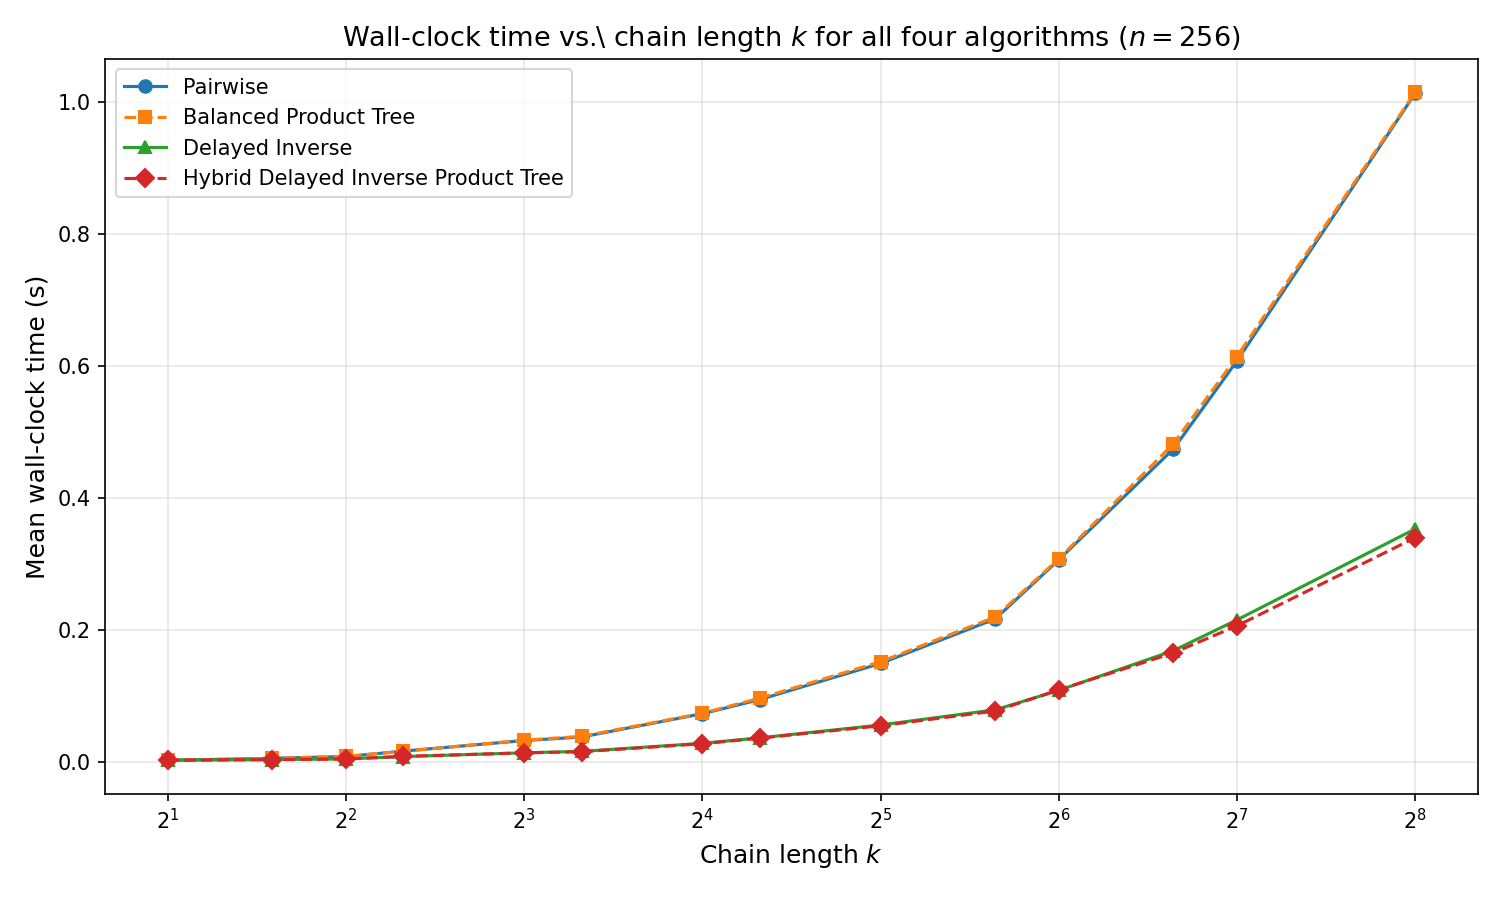
\includegraphics[width=\textwidth]{image.png}
    \caption{Wall-clock time vs.\ chain length $k$ for all four algorithms, with fixed operand size $n = 256$.}
    \label{fig:exp1_time}
\end{figure}

\subsubsection{Speedup Ratio}

Figure~\ref{fig:exp1_speedup} plots the measured speedup ratio (mean Pairwise time divided by mean Delayed Inverse time) alongside the theoretical transform-count ratio $\frac{3(k-1)}{k+1}$. The measured speedup broadly tracks the theoretical prediction and approaches the asymptotic limit of $3\times$ as $k$ grows.

The measured ratio consistently exceeds the theoretical curve at moderate $k$. This is expected: the theoretical ratio $\frac{3(k-1)}{k+1}$ counts only transforms, but the Pairwise algorithm also incurs overhead from repeatedly allocating and populating intermediate coefficient vectors between each INTT and the subsequent NTT. The Delayed Inverse avoids this overhead entirely by remaining in the spectral domain. At large $k$, this constant-factor advantage is diluted and the ratio converges toward the transform-count prediction.

\begin{figure}[htbp]
    \centering
    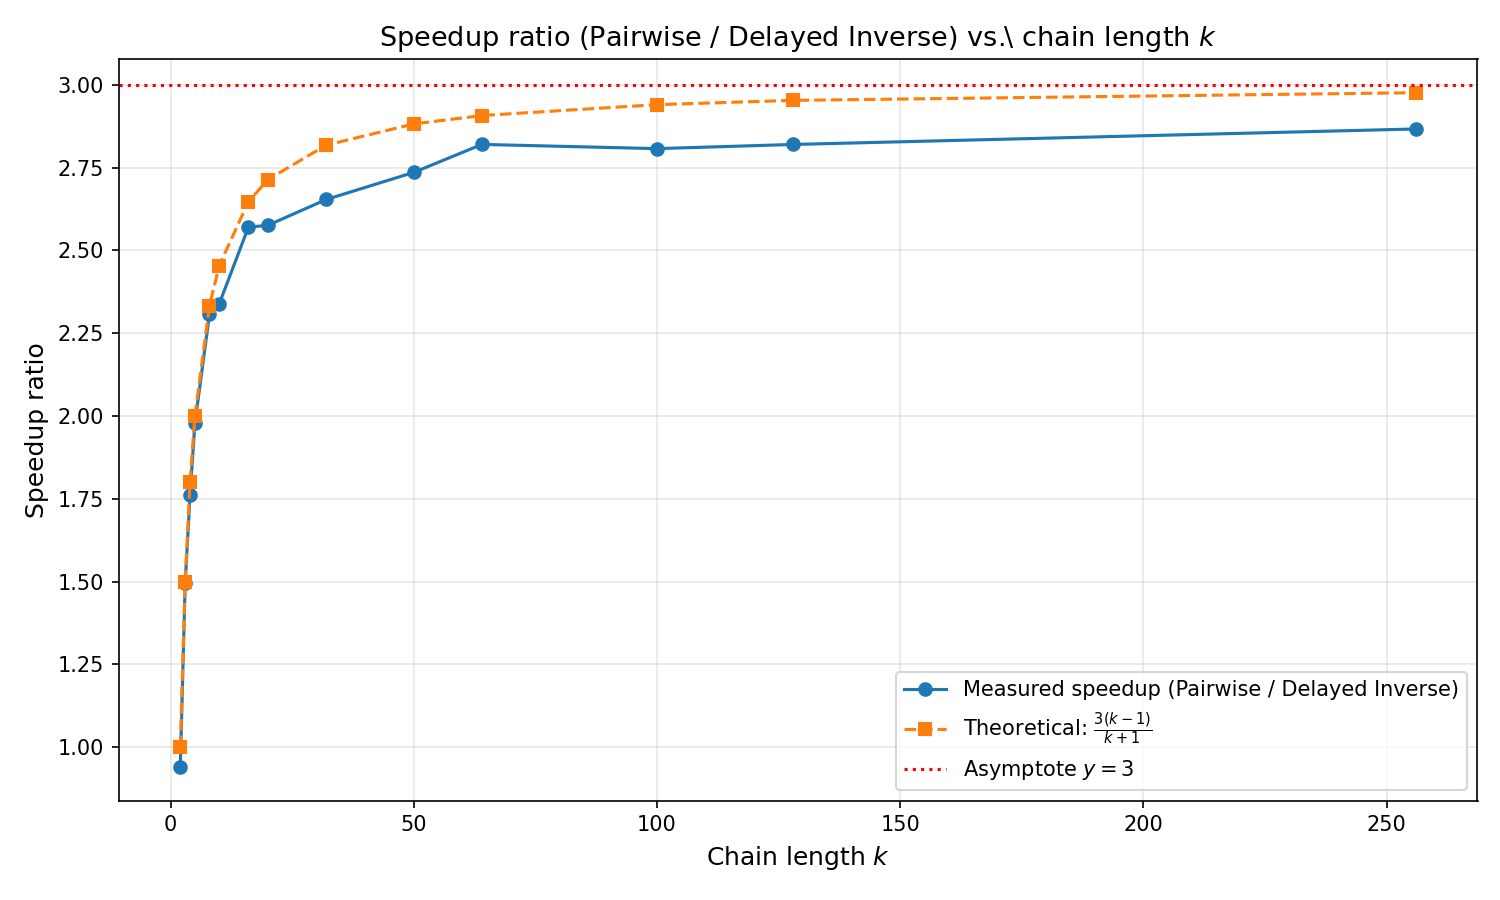
\includegraphics[width=\textwidth]{image (1).png}
    \caption{Speedup ratio (Pairwise / Delayed Inverse) vs.\ chain length $k$, compared to the theoretical transform-count ratio $\frac{3(k-1)}{k+1}$ and its asymptote $y = 3$.}
    \label{fig:exp1_speedup}
\end{figure}

\subsubsection{Timing Summary}

Table~\ref{tab:exp1_times} lists the mean wall-clock times (in milliseconds) for all four algorithms across each tested chain length, along with the measured and theoretical speedup.

\begin{table}[H]
\centering
\small
\begin{tabular}{r r r r r r r}
\hline
$k$ & Pairwise & Balanced PT & Delayed Inv. & Hybrid DI PT & Speedup & Theoretical \\
 & (ms) & (ms) & (ms) & (ms) & (meas.) & \\
\hline
2 & 2.8 & 2.9 & 3.0 & 2.9 & 0.94$\times$ & 1.00$\times$ \\
3 & 5.8 & 5.6 & 3.9 & 3.8 & 1.50$\times$ & 1.50$\times$ \\
4 & 8.5 & 8.7 & 4.8 & 4.8 & 1.76$\times$ & 1.80$\times$ \\
5 & 16.7 & 16.5 & 8.5 & 8.8 & 1.98$\times$ & 2.00$\times$ \\
8 & 32.7 & 33.3 & 14.2 & 14.0 & 2.31$\times$ & 2.33$\times$ \\
10 & 38.1 & 39.1 & 16.3 & 15.8 & 2.34$\times$ & 2.45$\times$ \\
16 & 73.4 & 74.1 & 28.6 & 27.9 & 2.57$\times$ & 2.65$\times$ \\
20 & 94.8 & 96.9 & 36.8 & 36.4 & 2.58$\times$ & 2.71$\times$ \\
32 & 149.5 & 152.1 & 56.3 & 55.1 & 2.65$\times$ & 2.82$\times$ \\
50 & 217.0 & 219.9 & 79.3 & 77.6 & 2.74$\times$ & 2.88$\times$ \\
64 & 306.5 & 308.1 & 108.7 & 109.4 & 2.82$\times$ & 2.91$\times$ \\
100 & 474.4 & 482.4 & 169.0 & 165.5 & 2.81$\times$ & 2.94$\times$ \\
128 & 607.7 & 614.3 & 215.5 & 206.5 & 2.82$\times$ & 2.95$\times$ \\
256 & 1012.8 & 1014.5 & 353.3 & 339.9 & 2.87$\times$ & 2.98$\times$ \\
\hline
\end{tabular}
\caption{Mean wall-clock time (ms) per algorithm and chain length $k$ ($n = 256$, 95 timed trials each). Speedup is the ratio of Pairwise to Delayed Inverse mean times.}
\label{tab:exp1_times}
\end{table}


\FloatBarrier
\subsection{Experiment 2: General Delayed Inverse Algorithm}


In this experiment we evaluate the General Delayed Inverse Algorithm described in Section~4.2. The setting differs from Experiment~1 in two key respects. First, polynomial coefficients are sampled from $[0, B)$ with $B = 2^{16}$, so intermediate products can exceed any single NTT-friendly prime; multiple CRT moduli are required. Second, only two algorithms are compared, those being General Pairwise ($3c(k-1)$ transforms) and General Delayed Inverse ($c(k+1)$ transforms), where $c$ is the number of CRT moduli needed to represent the product exactly. The theoretical speedup ratio $\frac{3(k-1)}{k+1}$ is the same as in the fixed-ring setting, but the constant factor from CRT reconstruction means the measured ratio may deviate slightly for larger $c$.

The operand size is fixed at $n = 256$. Chain lengths $k \in \{2, 3, 4, 5, 8, 10, 16\}$ are tested. Polynomial coefficients are sampled uniformly from $[0, 2^{16})$. The number of CRT moduli $c$ is chosen minimally for each $k$ so that $\prod_{j=0}^{c-1} q_j \geq n^{k-1} B^k$, as required by Proposition~4.1.

\subsubsection*{CRT Moduli and Roots of Unity}

The six NTT-friendly primes used are listed in Table~\ref{tab:exp2_moduli}. All primes satisfy $512 \mid q_j - 1$, guaranteeing the existence of a primitive $2n = 512$-th root of unity for $n = 256$. The first modulus is the 64-bit Goldilocks prime; the remaining five are the largest 63-bit primes satisfying this divisibility condition. For each modulus $q_j$ with primitive root $g$, the value $\psi_j = g^{(q_j - 1)/512} \bmod q_j$ satisfies $\psi_j^{256} \equiv -1 \pmod{q_j}$, as verified at runtime.

\begin{table}[htbp]
\centering
\small
\begin{tabular}{c r c r}
\hline
$j$ & Modulus $q_j$ & Prim.\ root $g$ & $\psi_j$ \\
\hline
0 & $2^{64} - 2^{32} + 1$ & 7  & 1803076106186727246 \\
1 & 9223372036854758401   & 7  & 8120564366590232957 \\
2 & 9223372036854747649   & 13 & 3345749197117459333 \\
3 & 9223372036854739969   & 11 & 5916304675994044514 \\
4 & 9223372036854739457   & 3  & 1511701938561174611 \\
5 & 9223372036854711809   & 3  & 251082263633788300  \\
\hline
\end{tabular}
\caption{CRT moduli used in Experiment~2. All satisfy $512 \mid q_j - 1$ and $\psi_j^{256} \equiv -1 \pmod{q_j}$.}
\label{tab:exp2_moduli}
\end{table}

\subsubsection*{Transform Count Verification}

For every $(k, c)$ pair tested, the instrumented counters confirmed the theoretical transform counts on every trial: General Pairwise required exactly $3c(k-1)$ transforms and General Delayed Inverse required exactly $c(k+1)$ transforms. No deviations were observed. Correctness was also verified on every trial by asserting that both algorithms produced identical coefficient vectors after CRT reconstruction via Garner's algorithm~\cite{garner1959residue}.

\subsubsection*{Wall-Clock Time}

Figure~\ref{fig:exp2_time} shows the mean wall-clock time for both algorithms as a function of chain length $k$. At $k = 2$, both algorithms use the same number of transforms ($3c(k-1) = c(k+1) = 3c$), so no speedup is expected; the measured times are within noise of each other. For $k \geq 3$, General Delayed Inverse is consistently faster, with the gap widening as $k$ increases. The absolute times are larger than in Experiment~1 because of the additional CRT reconstruction cost (Garner's algorithm~\cite{garner1959residue} over multiple moduli), but this overhead is common to both algorithms.

\begin{figure}[htbp]
    \centering
    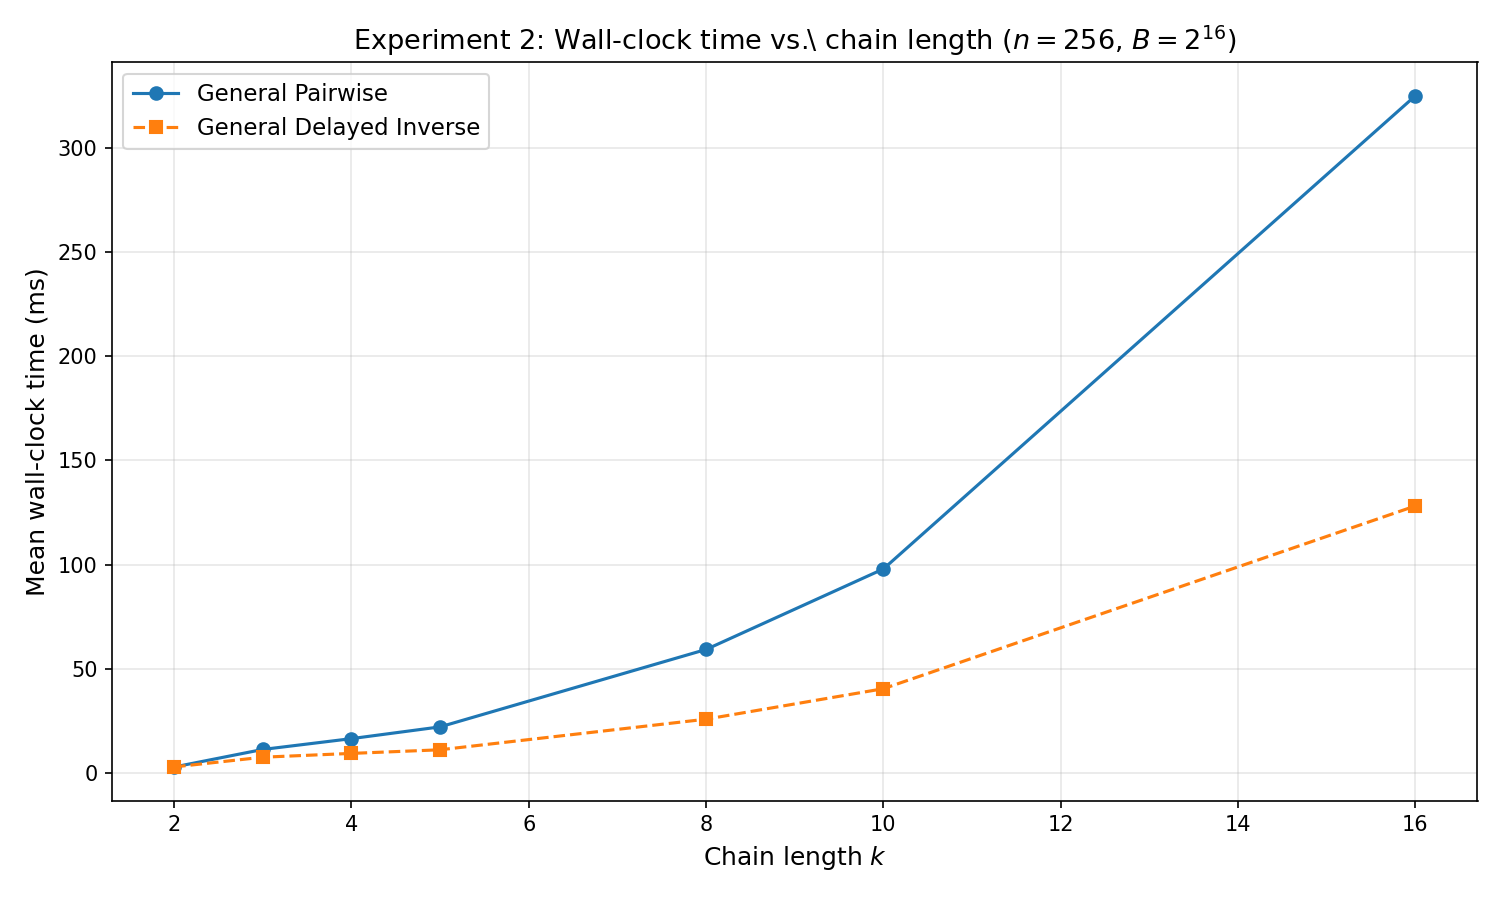
\includegraphics[width=\textwidth]{experiment2_time.png}
    \caption{Wall-clock time vs.\ chain length $k$ for General Pairwise and General Delayed Inverse ($n = 256$, $B = 2^{16}$).}
    \label{fig:exp2_time}
\end{figure}

\subsubsection*{Speedup Ratio}

Figure~\ref{fig:exp2_speedup} plots the measured speedup ratio alongside the theoretical prediction $\frac{3(k-1)}{k+1}$. The measured values track the theoretical curve closely. At $k = 16$ the gap is slightly wider (2.54$\times$ measured vs.\ 2.65$\times$ theoretical); this is consistent with the CRT reconstruction overhead, which is a constant cost shared by both algorithms but not captured by the transform-count ratio.

\begin{figure}[htbp]
    \centering
    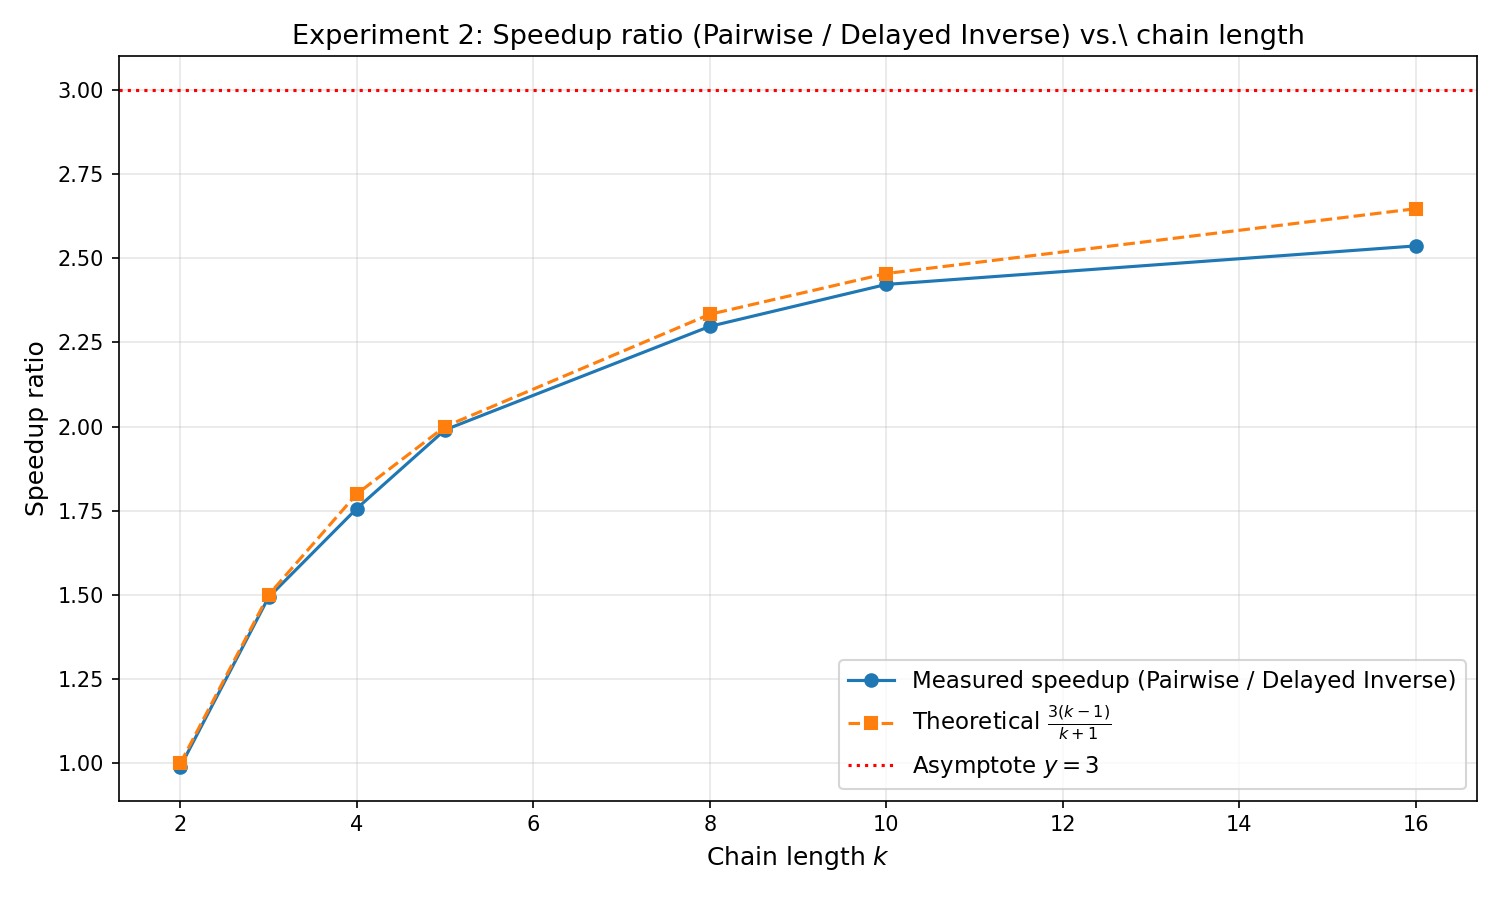
\includegraphics[width=\textwidth]{experiment2_speedup.png}
    \caption{Measured speedup ratio (General Pairwise / General Delayed Inverse) vs.\ $k$, compared to the theoretical transform-count ratio $\frac{3(k-1)}{k+1}$ and its asymptote $y = 3$.}
    \label{fig:exp2_speedup}
\end{figure}

\subsubsection*{Timing Summary}

Table~\ref{tab:exp2_times} lists the mean wall-clock times, CRT moduli counts, transform counts, and speedup ratios for all tested chain lengths.

\begin{table}[H]
\centering
\small
\begin{tabular}{r r r r r r r r}
\hline
$k$ & $c$ & PW transforms & DI transforms & PW (ms) & DI (ms) & Speedup & Theoretical \\
\hline
2 & 1 & $3$ & $3$ & 2.8 & 2.9 & 0.99$\times$ & 1.00$\times$ \\
3 & 2 & $12$ & $8$ & 11.3 & 7.5 & 1.49$\times$ & 1.50$\times$ \\
4 & 2 & $18$ & $10$ & 16.5 & 9.4 & 1.76$\times$ & 1.80$\times$ \\
5 & 2 & $24$ & $12$ & 22.1 & 11.1 & 1.99$\times$ & 2.00$\times$ \\
8 & 3 & $63$ & $27$ & 59.3 & 25.8 & 2.30$\times$ & 2.33$\times$ \\
10 & 4 & $108$ & $44$ & 97.9 & 40.4 & 2.42$\times$ & 2.45$\times$ \\
16 & 6 & $270$ & $102$ & 325.1 & 128.2 & 2.54$\times$ & 2.65$\times$ \\
\hline
\end{tabular}
\caption{Experiment 2: mean wall-clock time (ms) for General Pairwise and General Delayed Inverse ($n=256$, $B=2^{16}$, 95 timed trials). $c$ = CRT moduli count; PW $=3c(k-1)$, DI $=c(k+1)$ transform counts.}
\label{tab:exp2_times}
\end{table}



\section{Application: Mass RSA Key Auditing}

Security audits of large TLS certificate databases check whether any two RSA public keys share a prime factor --- a condition that immediately yields a complete factorisation of both moduli~\cite{heninger2012mining}. The standard algorithm builds a \emph{product tree} over the full collection of moduli and a corresponding \emph{remainder tree} to evaluate $\gcd(N_i,\, \prod_{j \neq i} N_j)$ for each modulus $N_i$~\cite{bernstein2004smooth}. At the core of both trees is the repeated multiplication of large integers. We show that the General Delayed Inverse Algorithm applies directly to this computation.

\subsection*{Integers as Polynomials with Integer Coefficients}

A $b$-bit RSA modulus $N$ can be written in a base-$2^w$ positional representation as
$$N = \sum_{j=0}^{d-1} n_j\, 2^{wj}, \qquad n_j \in [0,\, 2^w),$$
where $d = \lceil b/w \rceil$. Identifying $x = 2^w$, this is precisely the evaluation at $x = 2^w$ of the polynomial
$$N(x) = \sum_{j=0}^{d-1} n_j\, x^j \;\in\; \mathbb{Z}[x].$$
For RSA-2048 with $w = 64$, each modulus corresponds to a degree-$31$ polynomial with bounded integer coefficients $n_j \in [0,\, 2^{64})$, and $B = 2^{64}$.

Integer multiplication is then polynomial multiplication evaluated at the base:
$$N_i \cdot N_j \;=\; N_i(x) \cdot N_j(x)\big|_{x=2^w}.$$
This identification is the foundation of NTT-accelerated multi-precision arithmetic~\cite{schonhage1971}. Crucially, it means the product chain $N_1 \cdot N_2 \cdots N_k$ is exactly a product chain of degree-$(d{-}1)$ polynomials with bounded integer coefficients --- the setting of the General Delayed Inverse Algorithm.

\subsection*{Fixed-Ring Condition}

Choose $n$ to be the smallest power of two exceeding $(d-1)k$. For RSA-2048 ($d = 32$) and a batch of $k = 16$ moduli, the product polynomial has degree at most $31 \times 16 = 496 < 512$, so $n = 512$ suffices. Because the product degree is strictly less than $n$, no reduction modulo $x^n + 1$ occurs: the computation in $\mathbb{Z}[x]/(x^n+1)$ recovers the exact polynomial product, and evaluating at $x = 2^{64}$ recovers the exact integer product. All $k$ multiplications share the same ring, so the fixed-ring condition is satisfied.

\subsection*{Transform Count and CRT Moduli}

With $B = 2^{64}$, $n = 512$, and $k = 16$, the bound on product coefficients is
$$n^{k-1} B^k = 512^{15} \cdot \left(2^{64}\right)^{16} = 2^{135} \cdot 2^{1024} = 2^{1159}.$$
Using 63-bit NTT-friendly primes, this requires $c = \lceil 1159/63 \rceil = 19$ CRT moduli. The General Delayed Inverse then replaces the $3c(k-1) = 855$ transforms of a pairwise approach with $c(k+1) = 323$ transforms, a speedup of
$$\frac{3(k-1)}{k+1} = \frac{45}{17} \approx 2.65\times.$$

\subsection*{Deployment Context}

Internet-scale RSA audits routinely process tens of millions of public keys. Heninger et al.~\cite{heninger2012mining} applied batch GCD to approximately 7.1 million TLS certificates and 6.2 million SSH host keys, finding that 0.2\% of TLS hosts shared a prime factor with another host. The product tree at the core of this computation multiplies RSA moduli in a hierarchical chain; the General Delayed Inverse Algorithm reduces the NTT cost at every node of the tree where the fan-in is $k \geq 3$. At $k = 16$ per node, still practical for in-memory computation on modern hardware, the optimization delivers a $2.65\times$ reduction in transform operations across the most compute-intensive phase of the audit.

\section{Conclusion}

We have presented the Delayed Inverse Algorithm, a simple but effective optimization for computing polynomial product chains over NTT-friendly rings. By deferring the inverse transform and performing all intermediate multiplications as Hadamard products in the spectral domain, the algorithm reduces the number of transforms from $3(k-1)$ to $k+1$, yielding a speedup ratio of $\frac{3(k-1)}{k+1}$ that approaches $3\times$ as the chain length grows. We further presented the Hybrid Delayed Inverse Product Tree, which achieves the same transform savings while making use of parallel architecture.

Our experimental results over the Goldilocks prime confirm the theoretical transform counts exactly and demonstrate measured speedups consistent with the predicted ratio. The optimization is applicable wherever polynomial product chains are evaluated over a fixed quotient ring with an NTT-friendly modulus --- a condition satisfied in mass RSA key auditing~\cite{heninger2012mining}, where RSA moduli are represented as polynomials with integer coefficients and multiplied in batches as part of a product-tree-based batch GCD computation.

The key limitation of the approach is that it does not extend to settings where intermediate products grow in degree, such as general integer or arbitrary polynomial multiplication. In such cases, the NTT size must increase at each step, and the intermediate inverse-forward cancellation no longer applies.

Future work includes benchmarking in production cryptographic libraries written in lower-level languages, evaluating the parallel performance of the Hybrid variant on multi-core and GPU architectures, and investigating whether analogous transform-deferral strategies apply to other spectral methods beyond the NTT.

\begin{thebibliography}{99}

% --- Direct citations currently marked [?] ---

\bibitem{bos2018kyber}
J.~Bos, L.~Ducas, E.~Kiltz, T.~Lepoint, V.~Lyubashevsky, J.~M. Schanck,
P.~Schwabe, G.~Seiler, and D.~Stehl\'e,
``{CRYSTALS--Kyber}: A {CCA}-secure module-lattice-based {KEM},''
in \emph{2018 IEEE European Symposium on Security and Privacy (EuroS\&P)},
2018, pp.~353--367.

\bibitem{ducas2018dilithium}
L.~Ducas, E.~Kiltz, T.~Lepoint, V.~Lyubashevsky, P.~Schwabe, G.~Seiler,
and D.~Stehl\'e,
``{CRYSTALS--Dilithium}: A lattice-based digital signature scheme,''
\emph{IACR Transactions on Cryptographic Hardware and Embedded Systems},
vol.~2018, no.~1, pp.~238--268, 2018.


\bibitem{heninger2012mining}
N.~Heninger, Z.~Durumeric, E.~Wustrow, and J.~A. Halderman,
``Mining your {Ps} and {Qs}: Detection of widespread weak keys in network devices,''
in \emph{Proc. 21st USENIX Security Symposium},
USENIX Association, 2012, pp.~205--220.

% --- Closest prior work (Related Work) ---

\bibitem{saldamli2007spectral}
G.~Saldaml{\i} and \c{C}.~K. Ko\c{c},
``Spectral modular exponentiation,''
in \emph{18th IEEE Symposium on Computer Arithmetic (ARITH 2007)},
2007, pp.~123--132.

% --- Foundational NTT / FFT (cite in Section 3.1 and Experimental Setup) ---

\bibitem{pollard1971fft}
J.~M. Pollard,
``The fast {F}ourier transform in a finite field,''
\emph{Mathematics of Computation}, vol.~25, no.~114, pp.~365--374, 1971.

\bibitem{cooley1965algorithm}
J.~W. Cooley and J.~W. Tukey,
``An algorithm for the machine calculation of complex {F}ourier series,''
\emph{Mathematics of Computation}, vol.~19, no.~90, pp.~297--301, 1965.

\bibitem{gentleman1966fft}
W.~M. Gentleman and G.~Sande,
``Fast {F}ourier transforms: For fun and profit,''
in \emph{Proc. November 7--10, 1966, Fall Joint Computer Conference (AFIPS '66)},
1966, pp.~563--578.

\bibitem{dummit2004abstract}
D.~S. Dummit and R.~M. Foote,
\emph{Abstract Algebra}, 3rd~ed.
John Wiley \& Sons, 2004.

\bibitem{garner1959residue}
H.~L. Garner,
``The residue number system,''
\emph{IRE Transactions on Electronic Computers},
vol.~EC-8, no.~2, pp.~140--147, Jun.\ 1959.

\bibitem{numpy}
C.~R. Harris et~al.,
``Array programming with {NumPy},''
\emph{Nature}, vol.~585, pp.~357--362, 2020.

\bibitem{bernstein2004smooth}
D.~J. Bernstein,
``How to find smooth parts of integers,''
manuscript, 2004.
Available at \url{https://cr.yp.to/factorization/smoothparts-20040510.pdf}

\bibitem{schonhage1971}
A.~Sch{\"o}nhage and V.~Strassen,
``Schnelle {M}ultiplikation gro{\ss}er {Z}ahlen,''
\emph{Computing}, vol.~7, no.~3--4, pp.~281--292, 1971.

\end{thebibliography}
\end{document}

